%%%%%%%%%%%%%%%%%%%%%%%%%%%%%%%%%%%%%%%%%
% baposter Landscape Poster
% LaTeX Template
% Version 1.0 (11/06/13)
%
% baposter Class Created by:
% Brian Amberg (baposter@brian-amberg.de)
%
% This template has been downloaded from:
% http://www.LaTeXTemplates.com
%
% License:
% CC BY-NC-SA 3.0 (http://creativecommons.org/licenses/by-nc-sa/3.0/)
%
%%%%%%%%%%%%%%%%%%%%%%%%%%%%%%%%%%%%%%%%%

%----------------------------------------------------------------------------------------
%	PACKAGES AND OTHER DOCUMENT CONFIGURATIONS
%----------------------------------------------------------------------------------------

\documentclass[portrait,a1paper,fontscale=0.4]{baposter} % Adjust the font scale/size here

\usepackage{graphicx} % Required for including images
\graphicspath{{figures/}} % Directory in which figures are stored

\usepackage{amsmath} % For typesetting math
\usepackage{amssymb} % Adds new symbols to be used in math mode

\usepackage{booktabs} % Top and bottom rules for tables
\usepackage{enumitem} % Used to reduce itemize/enumerate spacing
\usepackage{palatino} % Use the Palatino font
\usepackage[font=small,labelfont=bf]{caption} % Required for specifying captions to tables and figures
\usepackage{wrapfig} % Allows wrapping text around tables and figures
%\usepackage{subfig}
\usepackage{float}
\usepackage[it]{subfigure}
\usepackage{multicol} % Required for multiple columns
\setlength{\columnsep}{1.5em} % Slightly increase the space between columns
\setlength{\columnseprule}{0mm} % No horizontal rule between columns

%\usepackage{tikz} % Required for flow chart
%\usetikzlibrary{shapes,arrows} % Tikz libraries required for the flow chart in the template

\newcommand{\compresslist}{ % Define a command to reduce spacing within itemize/enumerate environments, this is used right after \begin{itemize} or \begin{enumerate}
\setlength{\itemsep}{1pt}
\setlength{\parskip}{0pt}
\setlength{\parsep}{0pt}
}

\definecolor{lightblue}{rgb}{0.145,0.6666,1} % Defines the color used for content box headers
\definecolor{col1}{rgb}{0.9,0.9,0.9}
\definecolor{col2}{rgb}{0.9,0.9,0.9}
\begin{document}

\begin{poster}
{
headerborder=closed, % Adds a border around the header of content boxes
colspacing=1em, % Column spacing
%bgColorOne=white, % Background color for the gradient on the left side of the poster
bgColorOne=col1,
%bgColorTwo=white, % Background color for the gradient on the right side of the poster
bgColorTwo=col2,
borderColor=lightblue, % Border color
headerColorOne=black, % Background color for the header in the content boxes (left side)
headerColorTwo=lightblue, % Background color for the header in the content boxes (right side)
headerFontColor=white, % Text color for the header text in the content boxes
boxColorOne=white, % Background color of the content boxes
textborder=roundedleft, % Format of the border around content boxes, can be: none, bars, coils, triangles, rectangle, rounded, roundedsmall, roundedright or faded
eyecatcher=false, % Set to false for ignoring the left logo in the title and move the title left
headerheight=0.1\textheight, % Height of the header
headershape=roundedright, % Specify the rounded corner in the content box headers, can be: rectangle, small-rounded, roundedright, roundedleft or rounded
headerfont=\Large\bf\textsc, % Large, bold and sans serif font in the headers of content boxes
%textfont={\setlength{\parindent}{1.5em}}, % Uncomment for paragraph indentation
linewidth=2pt % Width of the border lines around content boxes
}
%----------------------------------------------------------------------------------------
%	TITLE SECTION 
%----------------------------------------------------------------------------------------
%
{
\includegraphics[height=4em]{logo.png}} % First university/lab logo on the left
{\bf\textsc{Hierarchical Controller Architecture in Software Defined Networks}\vspace{0.5em}} % Poster title
{\textsc{\{ Gourav Khaneja, Sweta Seethamraju \& Praveen Kumar \} \hspace{12pt}}} % Author names and institution
{\hspace{40pt} 
\includegraphics[height=8em]{UIUC_logo.png}} % Second university/lab logo on the right

%----------------------------------------------------------------------------------------
%	OBJECTIVES
%----------------------------------------------------------------------------------------

\headerbox{Problem}{name=problem,column=0,row=0}{

Typical Control plane architecture in SDN involves multiple peer controllers, managing subset of network, but keeping a global view of the network.

\begin{itemize}
    \item Replication of entire network state requires huge communication overhead: hinders scalability of the system
    \item Network inconsistency degrades the performance of control application
    \item Scalability of global network view itself
\end{itemize}

\vspace{0.3em} % When there are two boxes, some whitespace may need to be added if the one on the right has more content
}

%----------------------------------------------------------------------------------------
%	INTRODUCTION
%----------------------------------------------------------------------------------------

\headerbox{Proposed Solution}{name=solution,column=0,below=problem}{


\textbf{Switch Abstraction}
\begin{itemize}
    \item A controller creates an abstract switch representing the underlying managed network.
    \item A controller exposes "OpenFlow" API to manage the abstract switch by other (parent) controller.
    \item OpenFlow messages are translated between parent controller and underlying network. \\
\end{itemize}

\textbf{Hierarchical arrangement}
\begin{itemize}
    \item Controllers are arranged in a tree structure over the network using switch abstraction.
    \item Controllers do not keep a global view of network, but only the part which they control.
    \item Local application and network events are shielded from upper layer controllers.
\end{itemize}


\begin{center}
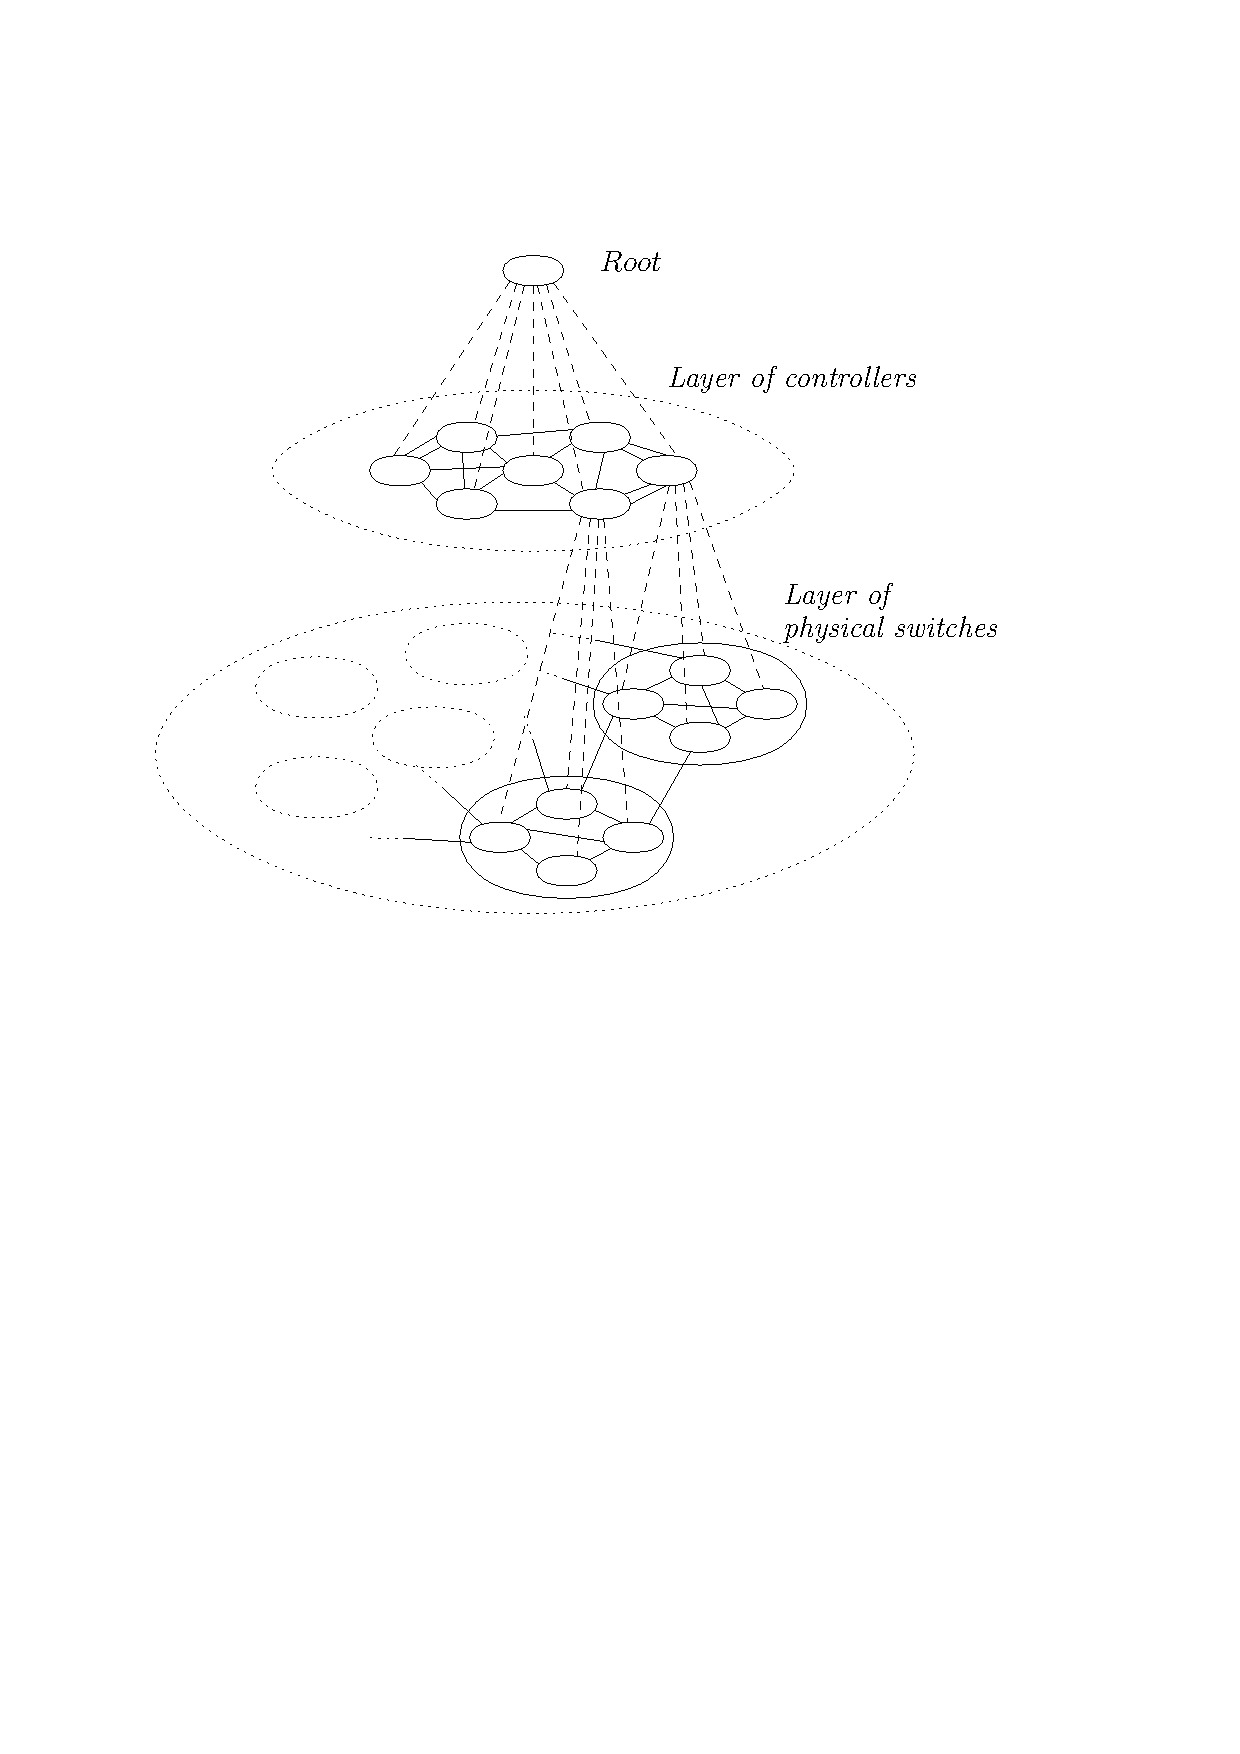
\includegraphics[scale=0.7]{hierarchy}
\captionof{figure}{Hierarchical arrangement of controllers}
\label{fig:hierarchy}
\end{center}

\textbf{Pros}
\begin{itemize}
    \item Reduces replication overhead
    \item Minimizes network inconsistency
    \item Enables smooth transition across management barriers
\end{itemize}
\textbf{Price we pay}  \\
Sub-optimality for inter-domain operations. How much is the deviation from optimality ?

}

\headerbox{EXPERIMENTAL SETUP}{name=exp,column=1,row=0}{
\begin{itemize}
%\item We simulated a dummy control application on both hierarchical and flat controller architectures, with same network topology and flow arrival distribution.
\item Flow data (6000 MapReduce jobs) was generated by sampling historical Hadoop traces on a 600 machine cluster at Facebook (1 million jobs). A dummy MapReduce application choses directory, map and reduce nodes randomly for each job.
\item Topology: 600 hosts connected through a network of 200 switches and 10 Gbps links. The cluster is divided into 10 equally-sized control domains.
\item TE-cum-routing control application: When a new flow arrives, it finds the path with minimum maximum utilization. If multiple such paths exist (which is frequently the case, due to a large network), shortest path (in term of number of hops) is chosen.
\end{itemize}
}

\headerbox{METRICS}{name=metrics,column=1,below=exp}{
\begin{itemize}
\item Path length (number of hops) of the routes assigned to flows.
\item Maximum link utilization of the path assigned to flows.
\item Communication overhead (number of messages exchanged between controllers) for setting up routes for flows.   
\end{itemize}

\begin{center}
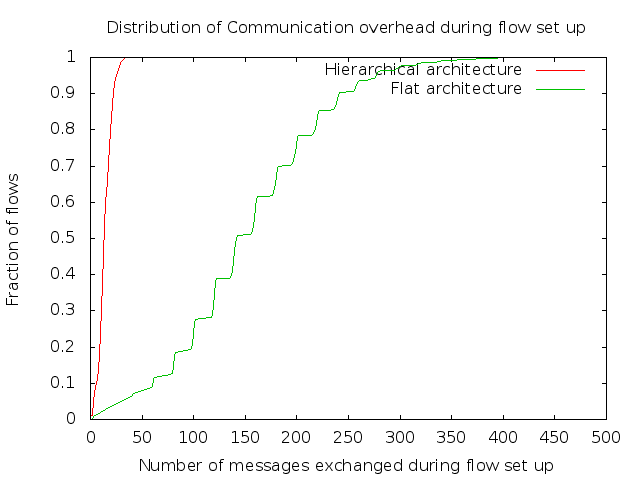
\includegraphics[scale=0.3]{msg}
\captionof{figure}{Per flow communication overhead}
\label{fig:msg}
\end{center}

\begin{multicols}{2}
\begin{minipage}{.5\textwidth}
\begin{center}
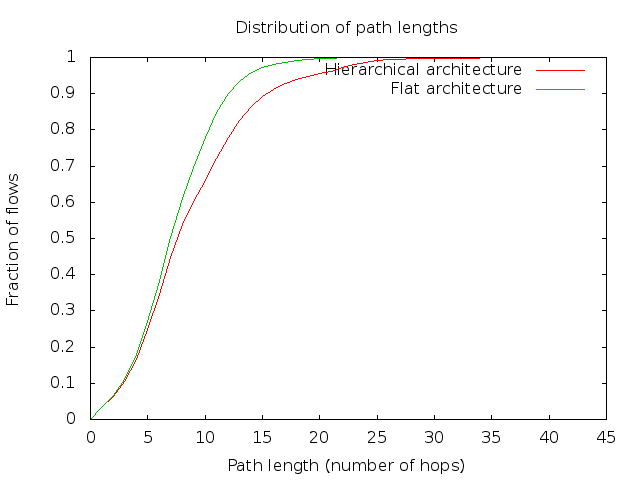
\includegraphics[scale=0.2]{path.png}
\captionof{figure}{Path length}
\label{fig:path}
\end{center}
\end{minipage}

\begin{minipage}{.5\textwidth}
\begin{center}
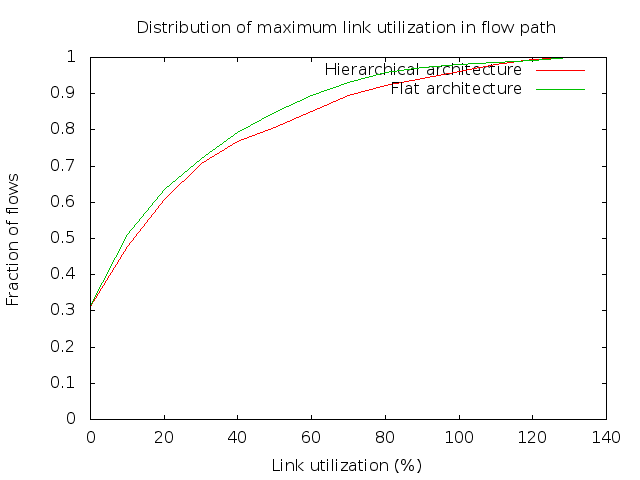
\includegraphics[scale=0.2]{util.png}
\captionof{figure}{Maximum link utilization}
\label{fig:util}
\end{center}
\end{minipage}
\end{multicols}


}

\headerbox{RESULTS}{name=results,column=1,below=metrics}{
    \begin{itemize}
        \item Reduces communication overhead by TODO (Figure \ref{fig:msg})
        \item Increases shortest path length by 17.4\% (Figure \ref{fig:path})
        \item Increases minimum maximum link utilization by 12.8\% (Figure \ref{fig:util}).
    \end{itemize}
Hierarchical architecture reduces communication overhead by an order of magnitude while compromising modestly on optimality
}


\headerbox{RESOURCES}{name=resources,column=1,below=results}{

https://github.com/MugiwaraLuffy/ACN/ \\
https://github.com/SWIMProjectUCB/SWIM

}

\end{poster}

\end{document}
